\begin{figure}
    \begin{center}
    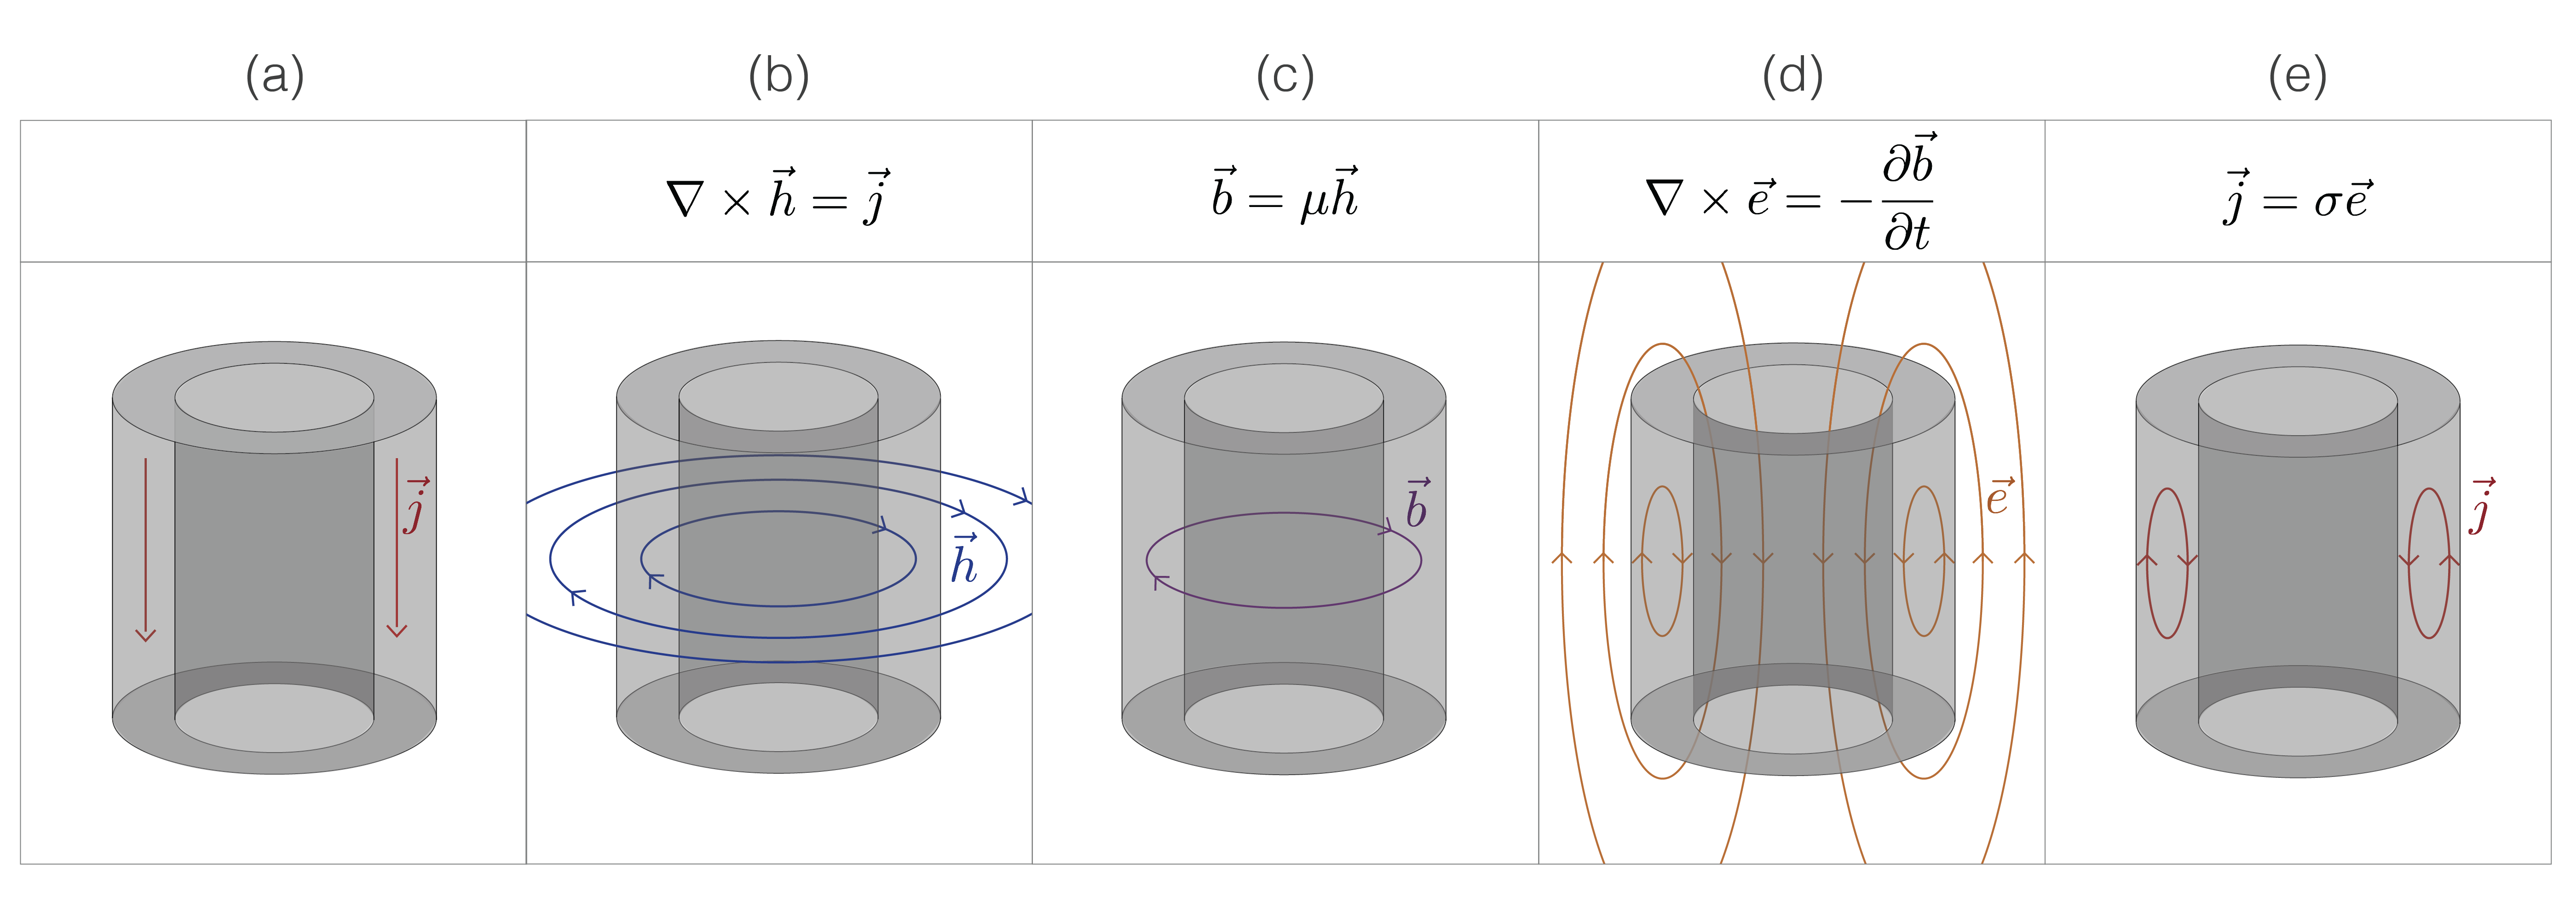
\includegraphics[width=\textwidth]{figures/em_casing/casing-mu-sketch.png}
    \end{center}
\caption{
    Sketch demonstrating how a vertical circulation of current can arise inside of a permeable casing in a top-casing TDEM experiment.
    A source current is applied and (a) currents flow downwards through the pipe. (b) Currents generate rotational magnetic fields according
    to Ampere's law. (c) Magnetic flux is concentrated in the permeable pipe according to the constitutive relation between $\vec{b}$ and $\vec{h}$.
    (d) The magnetic flux varies with time after shut-off, and the time-varying magnetic flux creates rotational electric fields according to Faraday's law.
    (e) Currents associated with those electric fields are concentrated in conductive regions of the model in accordance with Ohm's law.
}
\label{fig:casing-mu-sketch}
\end{figure}



